\newpage
\section[Herausforderungen bei der Implementierung von \gls{kryptografie} in Webanwendungen]{Herausforderungen bei der Implementierung von \gls{kryptografie} in Webanwendungen}\label{sec:Herausforderung-bei-der-implementierung-von-kryptografie-in-webanwendungen}
In den meisten Fällen überwiegt der Schutz, den \glsdisp{kryptografie}{Kryptografische} Methoden bieten, den Aufwand und die Probleme, die bei der Implementierung auftreten können. Nichtsdestotrotz wird man versuchen, die Probleme, wie \zb die in \autoref{subsec:performance-und-skalierbarkeitsprobleme} beschriebenen Leistungseinbußen oder die in \autoref{subsec:benutzerfreundlichkeit_und_usability-aspekte} erläuterte erschwerte Benutzbarkeit, zu beheben \bzw auf ein Minimum zu reduzieren.

\subsection{Performance- und Skalierbarkeitsprobleme}\label{subsec:performance-und-skalierbarkeitsprobleme}
Der in \autoref{subsubsec:HTTPS-Protocol} vorgestellte Vorteil der verschlüsselten Übertragung bringt allerdings auch einen Nachteil mit sich. Durch die Verschlüsselung der Daten verringert sich die Übertragungsrate und verlängert sich die Latenz der Übertragung\autocite[\pagef 5]{goldberg_comparison_nodate}, dies wird in \autoref{tab:HTTPS}\autocite[Übersetzt nach:][\pagef 5]{goldberg_comparison_nodate} dargestellt.

\begin{table}[htpb]
\caption[Parameter linearer Anpassungen an HTTP- und HTTPS-Übertragungen]{Parameter linearer Anpassungen an HTTP- und HTTPS-Übertragungen\footnotemark}
\label{tab:HTTPS}
\resizebox{\textwidth}{!}{%
\begin{tabular}{l|ll|ll}
                                                         & \multicolumn{2}{l|}{Transferrate (bytes/ms)} & \multicolumn{2}{l}{Latenz (ms)} \\ \cline{2-5} 
Server                                                   & Netscape             & Mircosoft             & Netscape       & Microsoft      \\ \hline
Unsicher                                                 & 946                  & 829                   & 4.5            & 19.0           \\
\begin{tabular}[c]{@{}l@{}}Sicher \\ 40 bit\end{tabular} & 730                  & 689                   & 3.6            & 3.9            \\
\begin{tabular}[c]{@{}l@{}}Sicher\\ 128 bit\end{tabular} & 736                  & 686                   & 25.0           & 5.1            \\ \hline
\end{tabular}%
}
\end{table}
\footnotetext{\cite[\pagef 5]{goldberg_comparison_nodate}}
Diese Daten sind allerdings aus dem Jahr 1998 und mittlerweile wurde \ac{HTTPS} verbessert, sodass der Performanceaufwand, der nötig ist um eine versclhüsselte Verbindung aufzubauen verringert wurde\autocite[\vglf][]{CloudfareWarumHTTPS:online}.

Neuere Versionen des \ac{TLS} \gls{algorithmus} bringen noch deutlichere Performance-Verbesserungen mit sich, da \uam nur ein \ac{TLS}-\gls{handshake}, behandelt in \autoref{par:tls_handshake_protocol}, benötigt wird, bzw. keiner, wenn bereits eine Verbindung zwischen \gls{client} und \gls{server} bestand\autocite[\vglf][]{CloudfareWarumHTTPS:online}.

Außerdem ist, trotz des Verdoppelns von CPU Geschwindigkeiten alle 18 Monate, ist die Performance von \ac{SSL} Maschinen noch immer ein Problem.\autocite[\vglf][\pagef 2]{cryptoeprint:2006/212}

Eine Möglichkeit, dies zu umgehen wäre es, das Entschlüsseln und Verifizieren des Zertifikates und der Signatur um die Identitaet des \glsdisp{client}{Clients} zu \gls{authentifizierung}{authentifizieren}, die Kommunikationsrichtung der \glspl{handshake} umzukehren, also das Verifizierun und Entschlüsseln der Daten \glsdisp{server}{Serverside} anstatt \glsdisp{client}{Clientside} zu berechnen\autocite[\vglf][\pagef 3]{cryptoeprint:2006/212}, wie die \autoref{fig:reverse_ssl_handshake}\autocite[\pagef 3]{cryptoeprint:2006/212} es darstellt.
\begin{figure}[htpb]
    \centering
    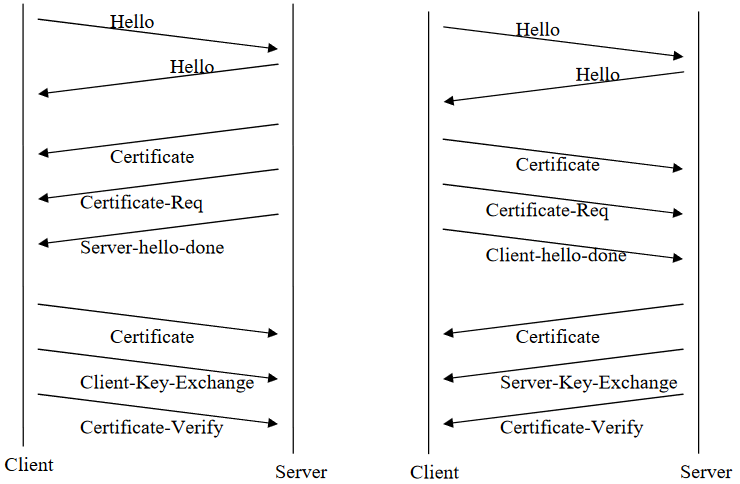
\includegraphics[width=0.75\linewidth]{abbildungen/reverse_ssl_handshake}
    \caption[Gegenüberstellung zwischen einem normalen SSL-Handshake und einem umgekehrten SSL-Handshake]{Gegenüberstellung zwischen einem normalen \ac{SSL}-\gls{handshake} und einem umgekehrten \ac{SSL}-\gls{handshake}\footnotemark}
    \label{fig:reverse_ssl_handshake}
\end{figure}
\footnotetext{\cite[\pagef 3]{cryptoeprint:2006/212}}
Da ein Großteil der Berechnungen für einen \ac{TLS}-\gls{handshake} während des Verifizieren der Zertifikate durchgeführt wird, wird die Laufzeit des \glspl{handshake} verbessert, wenn diese Berechnungen vom \gls{server} durchgeführt werden.

\subsection[Komplexität und Fehleranfälligkeit der Kryptografischen Methoden]{Komplexität und Fehleranfälligkeit der \glsdisp{kryptografie}{Kryptografischen} Methoden}\label{subsec:komplexitaet_und_fehleranfaelligkeit_der_kryptografie}

\subsubsection{Komplexität bei der Implementierung von Kryptografischen Methoden in Webanwendungen}\label{subsubsec:komplexitaet_bei_der_implementierung_von_Kryptografischen_methoden_in_webanwendungen}
Durch die Vielzahl an Lektüre zu den verschiedenen Verschlüsselungsmethoden\autocites[\zb][]{davies2011implementing} ist es heutzutage nicht mehr so kompliziert, \glsdisp{kryptografie}{Kryptografische} Methoden in Webanwendungen einzubauen, um Daten und die Anwendung als Ganzes zu sichern.
Gleichzeitig gibt es auch für viele Programmiersprachen mittlerweile vorgefertigte Methoden oder Packages, welche verschiedene \glsdisp{kryptografie}{Kryptografische} Methoden bereitstellen oder bündeln. So stellt die Programmiersprache \ac{JS} die Funktion \lstinline!digest(algorithm, data)! zur Verfügung, welche einen Datensatz nach einem der \ac{SHA}-\glspl{algorithmus} \ac{SHA}-1, \gls{SHA256}, \ac{SHA}-384 oder \ac{SHA}-512 verschlüsselt.\autocite[\vglf][]{SubtleCr83:online} Die \lstinline!decrypt(algorithm, key, data)! hingegen erlaubt es, mit RSA, beschrieben in \ac{RSA} oder \ac{AES} \glspl{algorithmus} zu verschlüsseln.

\subsubsection{Fehleranfälligkeit von Kryptografischen Methoden in Webanwendungen}\label{subsubsec:fehleranfälligkeit_von_Kryptografischen_methoden_in_webanwendungen}
Auch, wenn das \ac{TLS}-Protokoll schon viel analysiert wurde\autocites[Siehe \zb][]{krawczyk2013security, paulson1999inductive, dowling2015cryptographic, cremers2017comprehensive}, sind die gefundenen Mängel und Schwachstellen eher gering.\autocite[\vglf][\pagef 2239]{OPPLIGER20062238} 

\begin{definition}[\Acf{MITM}]
    \ac{MITM} bezeichnet nach \ac{RFC}\ \textnumero 2828\autocite[Übersetzt aus][\pagef 105]{rfc2828} eine Form des aktiven Lauschangriffs, bei dem der Angreifer kommunizierte Daten abfängt und selektiv verändert, um sich als sich als eine oder mehrere der an einer Kommunikationsbeziehung beteiligten Einheiten auszugeben.
\end{definition}

In einem typischen \ac{MITM} Angriff stellt sich das angreifende System so zwischen den \gls{client} und den \gls{server}, sodass es mit den \gls{client} und den \gls{server} unabhängig voneinander kommunizieren kann, die beiden Parteien aber den Eindruck behalten, sie würden direkt miteinander kommunizieren; eine Möglichkeit, sich einen \ac{MITM} Angriff vorzustellen ist es, als würde zwischen \gls{client} und \gls{server} ein \ac{SSL}/\ac{TLS} Proxy \gls{server} geschaltet sein.\autocite[\vglf][\pagef 4]{greenwood2014smv} Dadurch wissen weder der \gls{client} noch der \gls{server} über den \ac{MITM} bescheid.
\glsdisp{kryptografie}{Kryptografische Methoden} ändern bei einem \ac{MITM} Angriff nichts mehr an der Sicherheit, da der \ac{MITM} in der Verbindung integriert ist und alle Daten abfangen kann, so werden \zb Anmeldedaten dem \ac{MITM} sichtlich gemacht.\autocite[\vglf][\pagef 4]{greenwood2014smv}

\subsection{Benutzerfreundlichkeit und Usability-Aspekte}\label{subsec:benutzerfreundlichkeit_und_usability-aspekte}

\subsection{Abwägung von Sicherheitsanforderungen und Nutzerbedürfnissen}\label{subsec:abwaegung_von_sicherheitsanforderungen_und_nutzerbeduerfnissen}